\documentclass{astroedu-lab}

\begin{document}

\pagestyle{plain}

\begin{problem}{\huge Лабораторная работа 2.4.1\\\\Определение теплоты испарения\\\\жидкости\\\\Выполнил Жданов Елисей Б01-205}

\section{Цель работы:}

1) Измерение давления насыщенного пара жидкости при разной температуре

2) Вычисление по полученным данным теплоты испарения с помощью уравнения Клапейрона–Клаузиуса

\section{Оборудование:}

Термостат

Герметический сосуд, заполненный исследуемой жидкостью

Отсчетный микроскоп

\section{Теоретическая справка}

Для определения теплоты испарения будет использован косвенный метод, основанный на формуле Клапейрона–Клаузиуса.

\begin{equation}
	\frac{d P}{d T}=\frac{L}{T\left(V_2-V_1\right)}
\end{equation}

Вследствие высокой плотности воды положим изменение объемов равным(считая при атмосферном давлении пар идеальным газом).

\begin{equation}
	V=\frac{R T}{P}
\end{equation}

Подставляя выражение в уравнение Клапейрона–Клаузиуса, получим

\begin{equation}
	L=\frac{R T^2}{P} \cdot \frac{d P}{d T}=-R \frac{d(\ln P)}{d(1 / T)}
\end{equation}

\section{Экспериментальная установка}

\begin{figure}[!h]
	\centering
	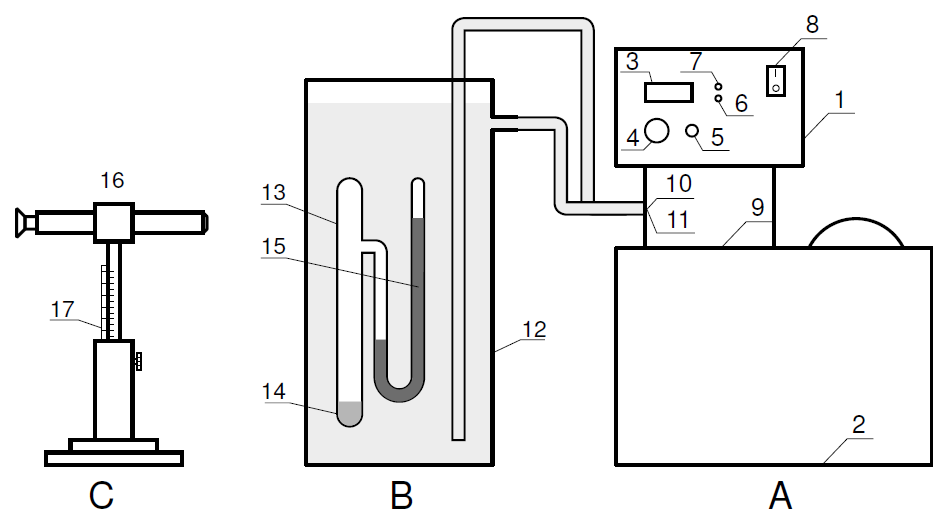
\includegraphics[width=0.9\textwidth]{установка.png}
	\label{fig:boiler}
\end{figure}

Над ней находится насыщенный пар (перед заполнением прибора воздух из него был откачан). Давление насыщенного пара определяется по ртутному манометру, соединенному с исследуемым объемом.

\section{Измерения, Обработка}

\begin{center}
\begin{tabular}{|c|c|c|c|}
\hline 
\multicolumn{2}{|c|}{$h_\text{ман}$, мм} & $\sigma, \frac{\text{мН}}{\text{К}}$ & T, $^\circ$C \\
\hline
188.0 & 188.0 & $(64.5 \pm 3.9)$ & 22\\
187.0 & 187.0 & $(64.0 \pm 3.9)$ & 30\\
185.5 & 186.0 & $(63.3 \pm 3.9)$ & 35\\
184.0 & 184.5 & $(62.5 \pm 3.9)$ & 40\\
182.5 & 183.0 & $(61.7 \pm 3.9)$ & 45\\
181.0 & 181.0 & $(60.8 \pm 3.8)$ & 50\\
179.0 & 179.5 & $(59.9 \pm 3.8)$ & 55\\
177.5 & 177.5 & $(59.0 \pm 3.8)$ & 60\\
\hline
\end{tabular}
\end{center}


Найдем угловые коэффициенты прямых для каждой установки по МНК.

\[
	a = \frac{<x_i y_i> - < x > < y_i >}{< x_i^2> - < x_i >^2}
\]

\[
	b = < \nu_i > - a < N_i >
\]

Также рассчитаем их погрешности

\begin{equation}
	S_a^2 = \frac{< x_i^2>}{< x_i^2 > - < x_i >^2} \cdot \frac{<  b_i - b > ^2}{n - 2}
\end{equation}


\begin{center}
	\Large $q(T)$
\end{center}

%\begin{figure}[!h]
%	\centering
%	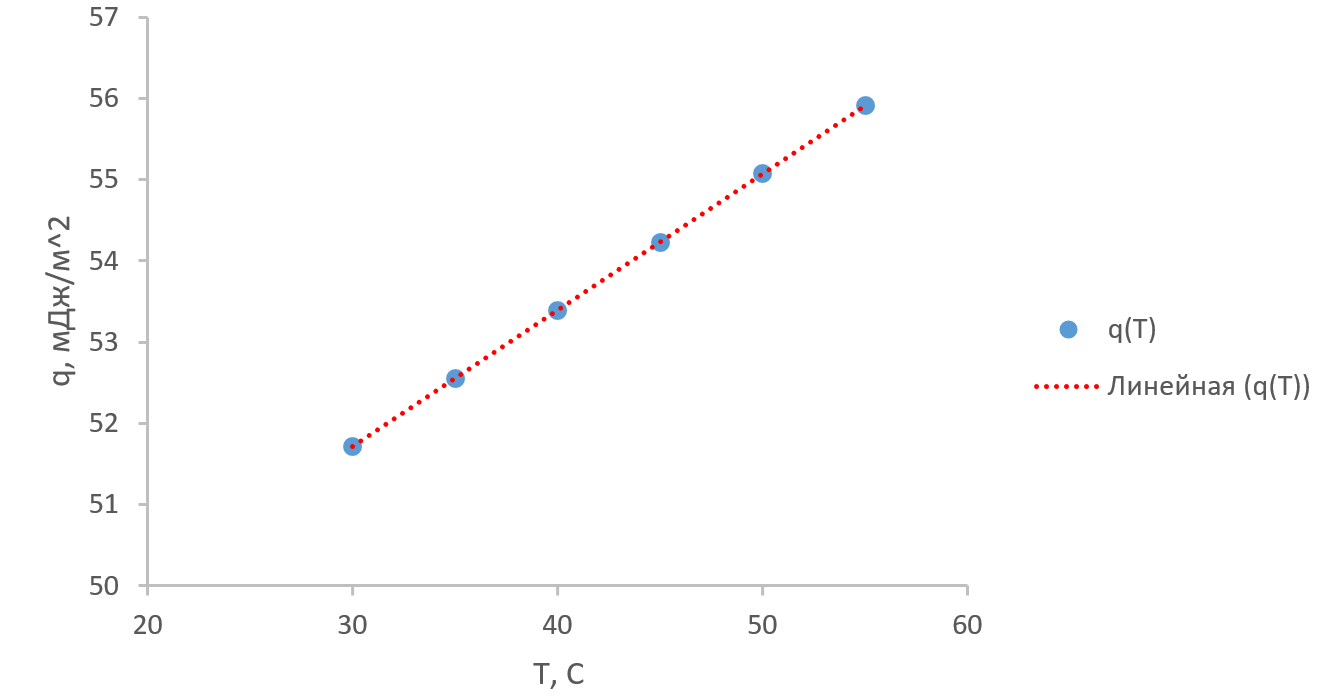
\includegraphics[width=1\textwidth]{2023-02-23_22-23-59.png}
%	\label{fig:boiler}
%\end{figure}

\section{Вывод}


\section{Ресурсы}

Расчет по МНК: метод-наименьших-квадратов.рф


\end{problem}
\end{document}